\documentclass{article}

\usepackage{hyperref}
\usepackage[dvipsnames]{xcolor}
\usepackage{listings}
\usepackage{amsmath}
\usepackage{tikz}

\title{All About Memory
}
\author{Ryan Baker}
\date{\today}

\definecolor{JadeGreen}{RGB}{91,158,62}
\lstdefinestyle{catppuccin}{
	backgroundcolor=\color{White},
	commentstyle=\color{Gray},
	numberstyle=\footnotesize\ttfamily\color{Gray},
	stringstyle=\color{JadeGreen},
	keywordstyle=\color{BurntOrange},
	basicstyle=\ttfamily\footnotesize\color{Black},
	breakatwhitespace=false,
	breaklines=true,
	captionpos=b,
	keepspaces=true,
	numbers=left,
	numbersep=5pt,
	showspaces=false,
	showstringspaces=false,
	showtabs=false,
	tabsize=4,
}
\lstset{style=catppuccin}

\hypersetup{
	colorlinks=true,
	hidelinks=false,
	linkcolor=RoyalBlue,
	citecolor=ForestGreen,
	filecolor=DarkOrchid,
	urlcolor=BurntOrange,
	runcolor=BrickRed,
	pdftitle={C++: From Code to Execution},
	pdfauthor={Ryan Baker},
}

\begin{document}

\maketitle
\tableofcontents
\pagebreak

\subsection*{Lecture Objectives}

\noindent By the end of this lecture, you should:
\begin{itemize}
	\item Understand pointers, references, and indirection
	\item Be able to use arrays to store and manipulate many variables
	\item Be able to reason about memory segments, and how they effect execution
\end{itemize}

\section{Pointers}

\noindent
Computers work with memory. Everything, from variables, to functions, to the actual machine code itself is stored in memory. Memory is extremely important. Pointers are tools to accessing and manipulating memory.

\subsection{Basics of Pointers}

\begin{itemize}
	\item What is a pointer?
	\begin{itemize}
		\item A pointer is a variable (an integer) that represents a memory address
	\end{itemize}
	\item Why use pointers? Pointer provide:
	\begin{itemize}
		\item Dynamic memory allocation and deallocation
		\item Passing large objects efficiently to functions
		\item Manipulation of memory at a low-level
	\end{itemize}
	\item Pointer syntax: \texttt{<type>* <name>}
	\begin{itemize}
		\item \textbf{Example:} \texttt{int* ptr;} declares a pointer to an \texttt{int}
		\item \textbf{Example:} \texttt{int* ptr = nullptr;} declares a \texttt{NULL} pointer to an \texttt{int}
		\begin{itemize}
			\item \texttt{nullptr} is a keyword that represents a null pointer value
			\item \texttt{NULL} is a pointer value that points to address 0 (invalid)
		\end{itemize}
	\end{itemize}
	\item Using pointers:
	\begin{itemize}
		\item Address-of operator: \texttt{\&}
		\begin{itemize}
			\item Use the address-of operator in front of a variable to get its address
			\item \texttt{std::cout << \&x << std::endl;} prints the address of \texttt{x}
			\item \texttt{int* ptr = \&x;} sets the value of \texttt{ptr} to the address of \texttt{x}
		\end{itemize}
		\item Dereference operator: \texttt{*}
		\begin{itemize}
			\item Use the dereference operator in front of a pointer to get the value
			\item \texttt{std::cout << *ptr << std::endl;} prints the value pointed to
			\item \texttt{int x = *ptr;} sets the value of \texttt{x} to the the memory pointed to by \texttt{ptr}
		\end{itemize}
		\item Together, the address-of and dereference operators allow you to access and manipulate memory with pointers
	\end{itemize}
\end{itemize}

\lstinputlisting[language=C++]{code/pointer.cpp}

\subsection{Pointer Arithmetic}

\begin{itemize}
	\item What is pointer arithmetic?
	\begin{itemize}
		\item Pointer arithmetic involves performing operations (such as addition or subtraction) on pointer variables, adjusting the memory address they reference based on the size of the data type they point to.
	\end{itemize}
	\item Pointer arithmetic in action:
	\lstinputlisting[language=C++]{code/parithmetic.cpp}
	\item \textbf{Key point:} Pointer arithmetic on \texttt{void*}s causes errors because \texttt{sizeof(void)} is undefined
\end{itemize}

\subsection{Pointers to Pointers}

\begin{itemize}
	\item Pointers are variables that represent memory addresses of other variables
	\item This means that a pointer can ``point to'' another pointer
	\begin{itemize}
		\item \texttt{sizeof(<pointer>)} = 8 (usually, for 64-bit systems)
		\begin{itemize}
			\item If you're working on a 32-bit system: \texttt{sizeof(<pointer>)} = 4
		\end{itemize}
	\end{itemize}
	\lstinputlisting[language=C++]{code/ptop.cpp}
\end{itemize}

\section{References}

\noindent
Every reference is just a pointer in disguise. They exist to help make working with pointers a bit easier.

\begin{itemize}
	\item What is a reference?
	\begin{itemize}
		\item A reference is a way to ``reference'' an existing variable
		\item There is no such thing as a \texttt{NULL} reference
		\item Think of references as aliases
	\end{itemize}
	\item Reference syntax: \texttt{<type>\& <name> = <variable>}
	\begin{itemize}
		\item \textbf{Example:} \texttt{int\& ref = x;} ``refers'' \texttt{ref} to \texttt{x}
	\end{itemize}
	\lstinputlisting[language=C++]{code/reference.cpp}
	\item\textbf{Example:} \texttt{increment(int x) \{...\}} vs. \texttt{increment(int\& x) \{...\}}
	\begin{itemize}
		\item When you pass by reference, the original value is modified
		\item When you pass by value (not reference), the original is untouched
	\end{itemize}
\end{itemize}

\section{Arrays}

\begin{itemize}
	\item What is an array?
	\begin{itemize}
		\item An array is a collection of variables stored contiguously
		\item Truly, an array is simply a pointer to its first element
	\end{itemize}
	\item When to use arrays?
	\begin{itemize}
		\item We often need to represent an entire collection of data, rather than creating many many variables, we can create an array
		\item \textbf{Example:} To represent the squares of a chess board, I could either create 64 variables: \texttt{int a1, int b1, ... int h8}, or use an array
	\end{itemize}
	\item Array syntax: \texttt{<type> <name>[<size>] = \{...\}}
	\begin{itemize}
		\item \textbf{Example:} \texttt{int chess\_board[64];}
	\end{itemize}
	\item Using arrays: \texttt{<name>[<index>]}
	\begin{itemize}
		\item Indices start at 0
		\item \textbf{Example:} \texttt{int square = chess\_board[32];}
		\item The square bracket (access) operator \texttt{[]} expands to a dereference:
		\begin{itemize}
			\item \texttt{arr[5]} $\rightarrow$ \texttt{*(arr + 5)} (Recall pointer arithmetic)
			\item This is why indices begin at 0
			\item To prove this: \texttt{arr[5] == 5[arr]}
		\end{itemize}
	\end{itemize}
	\lstinputlisting[language=c++]{code/access.cpp}
\end{itemize}

\section{Memory Segments}

\noindent
The memory that your operating system assigns to your executable is split up into different segments. Each segment is designed to hold a different type of data.

\begin{center}
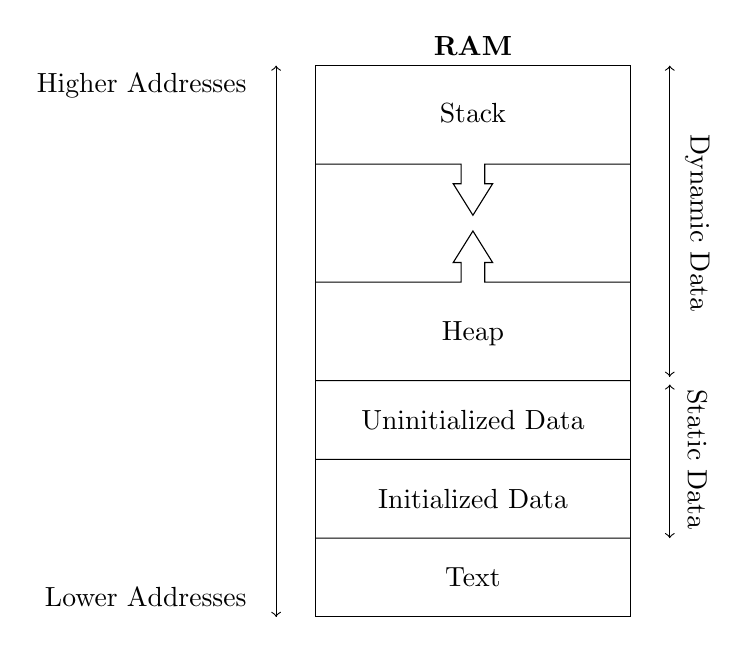
\begin{tikzpicture}

\draw
(0,0) -- ++(4,0) -- ++(0,7) -- ++(-4,0) -- (0,0)
;
\draw[->](-0.5,0) -- (-0.5,7);
\draw[->](-0.5,7) -- (-0.5,0);
\draw
(-0.75,6.75) node[left] {Higher Addresses}
(-0.75,0.25) node[left] {Lower Addresses}
(2,7) node[above] {\textbf{RAM}}
(0,1) -- (4,1) (2,0.5) node[] {Text}
(0,2) -- (4,2) (2,1.5) node[] {Initialized Data}
(0,3) -- (4,3) (2,2.5) node[] {Uninitialized Data}
(0,4.25) -- ++(1.85,0) -- ++(0,0.25) -- ++(-0.1,0) -- ++ (0.25,0.4) -- ++(0.25,-0.4) -- ++(-0.1,0) -- ++(0,-0.25) -- ++(1.85,0)
(0,5.75) -- ++(1.85,0) -- ++(0,-0.25) -- ++(-0.1,0) -- ++ (0.25,-0.4) -- ++(0.25,0.4) -- ++(-0.1,0) -- ++(0,0.25) -- ++(1.85,0)
(2,3.6) node[] {Heap}
(2,6.4) node[] {Stack}
;
\draw[->] (4.5,1)--(4.5,2.95) ;
\draw[->] (4.5,2.95)--(4.5,1) ;
\draw[->] (4.5,3.05) --(4.5,7);
\draw[->] (4.5,7) --(4.5,3.05);
\draw
(4.85,5) node[rotate=-90] {Dynamic Data}
(4.85,2) node[rotate=-90] {Static Data}
;
\end{tikzpicture}
\end{center}

\subsection{Text Segment}

\noindent
The text segment, a.k.a. the ``code'' segment, contains the machine code instructions to run your program. It is fixed in size and read-only. It also contains integer and string literals present in your code.

\subsection{Static Memory}

\noindent
Static memory is allocated at compile time and read directly from the executable. It contains global and static variables. This segment is divided into \textit{initialized} and \textit{uninitialized} data. The only difference is whether or not the variable has a compile-time initialized value.

\subsection{Heap Memory}

\begin{itemize}
	\item What is the heap?
	\begin{itemize}
		\item The heap is a memory segment that is variable in size and used for dynamic memory allocation.
        \item It gives the programmer direct control over memory, allowing you to allocate and deallocate memory manually.
        \item Think of it as a large pool of memory available for your program's use (though the term ``heap'' doesn't refer to this).
	\end{itemize}
	\item How to use the heap?
	\begin{itemize}
		\item Use the \texttt{new} operator to allocate memory:
		\begin{itemize}
		\item \texttt{int* ptr = new int(42);} Allocates an \texttt{int} with value 42
		\end{itemize}
		\item Use the \texttt{delete} operator to free memory:
		\begin{itemize}
		\item \texttt{delete ptr;} Frees the memory allocated to \texttt{ptr}
		\end{itemize}
	\end{itemize}
	\lstinputlisting[language=C++]{code/heap.cpp}
	\item \textbf{Memory leaks:}
	\begin{itemize}
		\item A memory leak occurs when memory is allocated on the heap but never freed, causing the program to consume more memory over time.
		\item Forgetting to deallocate memory with \texttt{delete} leads to memory leaks
		\item Dereferencing pointers that have been deleted is undefined behavior
		\item In short, manual memory management is somewhat error prone, especially in large or collaborative projects.
		\item Modern C++ provides alternatives to \texttt{new} and \texttt{delete} (covered in the future)
	\end{itemize}
	\lstinputlisting[language=C++]{code/leak.cpp}
\end{itemize}

\subsection{Stack Memory}

\noindent
The stack is where local variables and function arguments live. The name ``stack'' refers to how the structure operates. It works like a stack of books, where the last one placed down is the first one popped off.

\vspace{1em}
\noindent
Every time a new function is called, a stack frame is pushed onto the stack. This stack frame contains the function's arguments and local variables. You may only ever directly access the top stack frame, hence scoped variables. When the function returns, its stack frame is popped off the top.

\end{document}
